%!TEX root = ../LaTeX-cn.tex
\chapter{\tikzz\  繪圖*(編寫中,更新於\today)}
本章節極大地參考了 \tikzz\ 宏包手冊\cite{tikzmanual}。
\section{\tikzz\ 簡介}
``\tikzz \& PGF''(大多直接稱為\tikzz)是 \LaTeX\ 上與 PSTricks(PostScript Tricks) 齊名的繪圖擴展,而這兩者基本上是在你的 \LaTeX\ 文檔中繪製矢量圖的唯二選擇。Till Tantau\footnote{Till Tantau(1975---),德國呂貝克大學理論計算機科學研究處教授。他同時也是 \LaTeX\ 大名鼎鼎的幻燈片製作宏包 \pkg{beamer} 的開發者。} 開發了 \tikzz。

其中,``PGF'' 是 ``Portable Graphic Format''(便攜圖像格式)的縮寫,是整個繪圖系統的底層(或者後端);而 ``\tikzz'' 是 ``TikZ ist \emph{kein} 
Zeichenprogramm'' 的縮寫,即英文的 ``TikZ is not a drawing program''(“\tikzz\ 不是繪圖軟件”),則是系統的前端。Till 是仿造 GNU 的縮寫 ``GNU is Not Unix'' 這種遞歸式格式命名 \tikzz\ 的,他在文檔中也提及了這一點。

從 \tikzz\ 發佈穩定版以來,它的功能可以説涵蓋了文檔繪圖的絕大部分\textbf{科學繪圖場景}(我強調這一點,是因為我相信用它畫藝術設計圖的效率會很低)——對於研究工作者或者學生,這再好不過了。舉個例子:筆者在大學期間的計算機和統計課程的所有出圖都是由 \tikzz\ 繪製的。

\tikzz\ 的官方文檔,使用\texttt{texdoc tikz}命令調出。看的出來,Till 努力將文檔寫的生動有趣。如果不是篇幅實在有些長,相信你讀起來會很愉快。

\subsection{選擇 \tikzz\ 還是 PSTricks}
關於這兩者應該學哪一個,大家甚至展開聖戰;雖然沒有計算機行業 Vim 和 Emacs 聖戰那麼誇張,但是着實給不少想要學習 \LaTeX\ 繪圖的人帶來困擾\footnote{筆者就頗受困擾,所以都嘗試過。當年還有人把 Asymptote 也扯進這場聖戰,但筆者認為它的競爭力沒有那麼強。}。

筆者最後選擇了 \tikzz\ 。為什麼?相比 PSTricks,語法順暢,可讀性更高。易讀易寫,十分難得。至於誰的繪圖能力更強,我認為他們都已經涵蓋了你正常需要的範疇。所以,如果你仍然不確定的話,就去搜索一些他們各自的例子片段再決定吧。

\subsection{選擇 \tikzz\ 還是外部繪圖軟件}
為什麼選擇 \tikzz\ 而不是用外部繪圖軟件呢?一些理由:
\begin{itemize}
\item \textbf{繪製矢量圖}。外部繪圖為 pdf 矢量圖再用加載圖片的方式加載進來當然可以;但是很多情況下,切換軟件的時間成本與切換到另一個軟件的操作模式的思考成本是很高的。
\item \textbf{更小的體積}。相比加載外部繪圖,體積會小一些;雖然不是特別明顯。
\item \textbf{更易維護}。外部繪製的圖片需要你通過安裝相應的繪圖軟件進行維護;但是使用 \tikzz\ 繪圖,你只需要一台裝有 \LaTeX\ 核心和 \tikzz\ 宏包的設備。

千萬別小看這一點;很多時候你需要在別人的電腦上更改你的插圖。比如學術圈子裏,電腦上安裝有 \TeX\ Live 是一件稀鬆平常的事情;但是安裝有 GNUplot 繪圖,矢量圖編輯器?那可不一定。
\item \textbf{完全的文本文件}。如果你使用 git 之類的版本控制工具,你應該會明白這一條是什麼意思。不管你是將 \tikzz\ 代碼寫在主 tex 文檔中,還是另存到一份單獨的 tex 文檔,它們都是文本文件。如果用加載外部 pdf 的方式導入圖片,那想對它們進行版本控制簡直是一場災難。
\end{itemize}

\section{\tikzz\ 的輸入輸出}
\subsection{基本繪圖方式}
\tikzz\ 的基本繪圖方式有兩種:使用 \latexline{tikz} 命令,或者使用 \envi{tikzpicture} 環境。請注意,\RED{語句用分號結尾}。當然,你需要先加載 \pkg{tikz} 宏包,有時你還需要加載一些 \tikzz\ 的庫:
\begin{latex}
\usepackage{tikz}
% 加載庫:\usetikzlibrary{lib1, lib2, ...}
\end{latex}

兩個例子:
\begin{codeshow}
% 使用 \tikz 命令
\tikz{\draw (0,1) -- (1,0)}
% 使用 tikzpicture 環境
\begin{tikzpicture}
\draw (0,0) -- (1,1);
\end{tikzpicture}
\end{codeshow}

如果你使用 \TeX\ 而非 \LaTeX\ ,那麼請在 \latexline{tikzpicture} 和 \latexline{endtikzpicture} 之中使用 \tikzz\ 代碼。

\subsection{輸出圖像到獨立文件}
要輸出為\texttt{.svg}矢量文件,用於更多的插圖場合。需要在電腦安裝pdf2svg\footnote{\url{http://www.cityinthesky.co.uk/opensource/pdf2svg/}}。不過在\LaTeX 使用的場合,可以去掉下述的\texttt{convert}參數,以輸出\texttt{.pdf}格式的矢量文件。下例中的\texttt{multi=false}表示只輸出為單頁文件。

\begin{latex}
\documentclass[tikz,convert=pdf2svg,multi=false]{standalone}
% tikz package already loaded by 'tikz' option
\begin{document}
\begin{tikzpicture}
  \draw (0,0) -- (10,10);
  \draw (10,0) -- (0,10);
\end{tikzpicture}
\end{document}
\end{latex}

在編譯時如果是\xelatex ,還需要添加參數:
\begin{latex}
% 如果上例的文件名為 example.tex
xelatex -shell-escape example.tex
\end{latex}

\section{基礎幾何元素}
本節介紹 \tikzz\ 的基礎幾何元素,希望能夠幫助讀者較系統地進行學習。如果讀者希望通過例子入手,請參考\secref{sec:tikz-eg}。

\subsection{點與線段}
點和線是繪圖的基本要素。\tikzz\ 通過座標的方式指定點的位置,座標書寫在一對圓括號內;通過兩個短橫線“--”來連接點與點,形成線段。下例連續畫了兩段。\RED{為了簡潔,下文展示代碼時省略 tikzpicture 環境首尾}。
\begin{tikzshow}
\draw (0,0) -- (1,0) -- (2,0.5);
\end{tikzshow}

默認的單位長度是 1 cm。如果想要修改比例尺,或者調整線型、顏色等屬性參數,請參考\secref{sec:tikz-property}。極座標參考\secref{subsec:coord}。

\subsection{路徑}
命令 \latexline{path} 可以只創建路徑但不繪製;實質上,\latexline{draw} 命令就是 \latexline{path[draw]} 的簡寫形式。\latexline{fill} 命令也類似。

\subsection{\bz\ 曲線}
\tikzz\ 允許你使用 \tikzkw{.. controls <p1> and <p2> ..} 方式來指定\bz\ 曲線的兩個控制點。第二控制點可以省略;省略時,設為與第一控制點相同。
\begin{tikzshow}
\draw (0,0) .. controls (0.5,1) and (1.5,1) .. (2,0);
\end{tikzshow}

控制點並不會顯式地畫在圖中。為了幫助不熟悉 \bz\ 曲線的讀者理解,在此繪製一些輔助説明的點和線:
\begin{tikzshow}
\draw (0,0) .. controls (0.5,1) and (1.5,1) .. (2,0);
% Auxilary Points & Lines
\filldraw[black] (0,0) circle [radius=2pt] (0.5,1) circle [radius=2pt] (1.5,1) circle [radius=2pt] (2,0) circle [radius=2pt];
\draw[dashed] (0,0) -- (0.5,1);
\draw[dashed] (1.5,1) -- (2,0);
\end{tikzshow}

\subsection{矩形}
指定矩形的西南角點和東北角點,用 \tikzkw{rectangle} 命令連接:
\begin{tikzshow}
\draw (0,0) rectangle (2,1);
\end{tikzshow}

\subsection{圓與橢圓}
指定圓或者橢圓的中心,然後指明它半徑的參數\footnote{\texttt{circle (1cm)} 的寫法較陳舊,不建議再使用。橢圓繪製也請使用 \tikzkw{circle},而不是陳舊的 \tikzkw{ellipse}。}:
\begin{tikzshow}
\draw (0,0) circle [x radius=12pt, y radius=6pt];
\draw (2,0) circle [radius=0.5cm];
\end{tikzshow}

\subsection{圓弧與橢圓弧}
指定圓弧的起點,在選項中給出起始角度、終止角度和半徑,即可畫弧:
\begin{tikzshow}
\draw (2,0) arc [start angle=0, end angle=45, radius=2];
\draw (1,0) arc [start angle=0, end angle=270, x radius=1, y radius=.5];
\end{tikzshow}
你也可以不指定 \tikzkw{end angle} 而使用圓弧對應的圓心角 \tikzkw{delta angle}。 在繪製弧時使用極座標,請參考\secref{subsec:coord}。

\subsection{網格}
網格即為自動繪製的等距線:
\begin{tikzshow}
\draw[step=0.5,lightgray,thin] (0,0) grid (2,2);
\draw (1,1) circle [radius=.5];
\end{tikzshow}
默認的 \tikzkw{step} 是 1。 \tikzkw{xstep} 和 \tikzkw{ystep} 命令可分別指定沿兩個軸向的間距。

\subsection{拋物線*}
拋物線使用 \tikzkw{parabola} 繪製,並可使用 \tikzkw{bend} 指定拐點位置:
\begin{tikzshow}
\draw[help lines, xstep=1, ystep=2] (0,0) grid (3,4);
\draw (0,2) parabola[bend at end] (1,0);
\draw[xshift=1cm] (0,1) parabola (1,2);
\draw[xshift=2cm] (0,0) parabola bend (0.5,2) (1,0);
\draw[yshift=2cm] (0,0) parabola[bend pos=0.75] bend +(0,1) (1,0);
\draw[xshift=1cm, yshift=2cm] (0,0) -- (1,2) parabola cycle;
\draw[xshift=2cm, yshift=2cm] (0,0) parabola[parabola height=2cm] +(1,0);
\end{tikzshow}
其中 \tikzkw{xshift/yshift} 參考 \secref{subsubsec:shift}。拋物線的參數解釋如下:
\begin{para}
\item[bend at end] 或者 \tikzkw{bend at start},這樣拋物線是正常情況的一半。
\item[bend] 指定在何處設置拐點。
\item[bend pos=L] 在起點、終點連線的 L 分點處為基準設置拐點,比如上例為四分之三分點向上偏移 1 單位。
\item[cycle] 使用 \tikzkw{cycle} 結尾,自動直線連接首尾,形成閉合路徑。
\item[parabola height=H] 在起終點連線的二分之一分點處向上偏移 H 處設置拐點。
\end{para}

\subsection{正弦線與餘弦線*}
使用 \tikzkw{sin} 和 \tikzkw{cos} 繪製。

\section{座標與圖像}
\subsection{引言:畫筆位置}
\tikzz\ 中一個很重要的概念是畫筆,在一個常規的 \latexline{draw} 命令中,想象使用畫筆從頭到尾依次連接各個點。每次檢測到“--”這條繪製命令,\tikzz\ 都將移動畫筆位置並畫線。

\tikzz\ 提供了一種方法,可以在移動畫筆的同時不劃線。這個命令就是 \tikzkw{++}:
\begin{tikzshow}
\draw (0,0) -- (1,0) ++(0,1) circle [radius=.25] -- ++(-1,0) -- (0,0);
\end{tikzshow}

\tikzz\ 還提供了一個命令 \tikzkw{+},可以\textbf{臨時}偏移畫筆:
\begin{tikzshow}
\draw (0,0) -- (1,0) -- +(0,1) circle [radius=.25] -- +(-1,1) -- +(-1,0);
\end{tikzshow}

請仔細體會兩個命令的不同之處:單加號用於\uline{指代相對座標},而相對座標的基準點不會改變,直到指定新的絕對座標 ;雙加號用於\uline{移動畫筆},基準點的位置會隨之改變。

\subsection{指定座標}
\label{subsec:coord}
本節介紹瞭如何指定座標,包括直角座標、極座標,以及如何指定一個相對於已知點的座標。其他座標系也會在此介紹。

\subsubsection{直角座標與極座標}
通常會使用直角座標系(coordinate system)來標定座標位置,正如上一節所示。直角座標的格式是 \texttt{(x,y)},其中 $x$ 軸正向指向紙面右方,$y$ 軸正向指向紙面上方;而極座標的格式是 \texttt{(角度:\mbox{}距離)}。

實質上,上述座標的是隱式指定的;如果要顯式指定,格式如下例的第二行:
\begin{tikzshow}
\draw[red] (0,0) circle [radius=0.5] -- (30:1cm);
\draw (canvas cs: x=0, y=0) -- (canvas polar cs: radius=1cm, angle=60);
\end{tikzshow}

\subsubsection{相對已知點的座標}
大致有這麼幾種方法:
\begin{feai}
\item 使用上一節中的單加號或雙加號指令來指定相對位置;
\item 使用平移參數 \tikzkw{shift} (參考\secref{subsubsec:shift}內容);
\item 使用扭轉參數 \tikzkw{turn},它基於進入當前點的切線方向,這在繪製折線時很有用;
\item 使用 \pkg{calc} 庫支持的 \verb|($ ... $)| 指令進行計算。
\end{feai}

一個綜合上述方法的例子:
\begin{tikzshow}
\draw (0,0) circle[radius=1];
\draw (0,0) { [current point is local]-- ++(1,-1)} -- ++(0,-0.5); 
\draw[red] (0,0)
     -- ([shift=(90:.5cm)] 210:1cm)
     -- (210:1cm) -- cycle;
\draw[blue] (0,0) -- (1,0)
     -- ($ (1,0) + (120:1cm) $) -- cycle;
\draw[green] (0,0) -- (150:.5cm) -- ([turn]-45:.5cm)
     arc[start angle=105, delta angle=-135, radius=.5];
\end{tikzshow}
其中,選項 \tikzkw{current point is local} 表示當前花括號內的畫筆移動不會影響到外部的畫筆位置。

\subsubsection{三維座標系*}
通常 \tikzz\ 繪圖只需要用到平面座標,但它也支持三維座標系。

\tikzz\ 使用了名為 \texttt{xyz} 的座標系統來支持三維座標,因此調用是:
\begin{tikzshow}[thick]
\draw (0,0) -- (xyz cs: x=1);
\draw[red] (0,0) -- (0,1,0);
\draw[blue] (0,0) -- (0,0,1);
\end{tikzshow}

\subsubsection{重心座標系*}
重心座標系(barycentric coordinate system)指定一系列向量 $\overrightarrow{v_1}, \overrightarrow{v_2},\ldots,\overrightarrow{v_n}$,然後座標為 $(p_1,p_2,\ldots,p_n)$ 的點的位置是它們的線性組合向量對應的位置:
\[ \frac{p_1\overrightarrow{v_1}+p_2\overrightarrow{v_2}+\cdots+p_n\overrightarrow{v_n}}{p_1+p_2+\cdots+p_n} \]

一個例子(涉及的命令會在另外的章節介紹):
\begin{tikzshow}
\tikzset{small/.style={draw=none, circle, fill=#1!70, inner sep=1pt}}
\coordinate[label=above:A] (A) at (90:1cm);
\coordinate[label=below left:B] (B) at (210:1cm);
\coordinate[label=below right:C] (C) at (-30:1cm);
\draw (A) -- (B) -- (C) -- cycle;
\node[small=red] at (barycentric cs:A=0,B=0.3,C=0.7) {};
\node[small=blue] at (barycentric cs:A=0.5,B=0.5,C=0.5) {};
\node[small=green] at (barycentric cs:A=0.5,B=0.5,C=0.1) {};
\end{tikzshow}

\subsection{交點}
\label{subsec:intersection}
\tikzz\ 提供一種簡潔的座標交點控制,例如 \texttt{(<p1> -| <p2>)} 中,用短橫表示過 \texttt{p1} 的水平線、用豎線表示過 \texttt{p2} 的豎直線,這兩條線的交點就是該命令表示的點。類似還有命令 \tikzkw{|-} 。
\begin{tikzshow}
\draw (0,0) circle [radius=1cm] -- (30:1 |- 0,0) -- (30:1) -- cycle;
\end{tikzshow}

利用 \tikzz\ 的 \pkg{intersections} 庫,還可以尋找兩條路徑的交點:
\begin{tikzshow}
% \usetikzlibrary{intersections}
\path[name path=line1] (0,0) -- (1,1);
\path[name path=line2] (0,1) -- (1,0);
\draw[name intersections={of=line1 and line2, by=A}] (0,0) -- (A) -- (1,0);
\end{tikzshow}

有時路徑會有多個交點,這時你可以依次用 \texttt{intersection-1, 2, \ldots} 來指定它們。或者,你可以使用 \tikzkw{name} 選項代替上例的 \tikzkw{by},然後使用你的自定義名稱:
\begin{tikzshow}
\path[name path=line1] (-2,.25) -- (2,.25);
\draw[name path=circle] (0,0) circle [radius=.5];
\draw[name intersections={of=circle and line1, name=A}] (1,0) -- (A-1);
\draw (0,0) -- (A-2);
\end{tikzshow} 

用 \tikzkw{total} 可以存儲交點個數到一個宏命令,而 \tikzkw{sort by} 可以指定以相交路徑中的某一條來給交點排序\cite{tikzmanual}:
\begin{tikzshow}[scale=0.7]
\tikzset{small/.style={draw, circle, fill=#1!70, inner sep=2pt}}
\foreach \pathname/\offset/\color in {la/0cm/black,lb/3cm/red} {
    \tikzset{yshift=\offset}
    \draw[->,name path=la] (2,4) -- (0,0);
    \draw[->,name path=lb] (1,.5) .. controls (0,1) and +(-2,-1) .. (1.5,2)
         .. controls +(2,1) .. (1,3);
    \path[name intersections={of=la and lb, sort by=\pathname, name=inter, total=\s}] \foreach \i in {1,2,...,\s} {
        (inter-\i) node[small=\color,
        label=below right:\i] {}
    };
}
\end{tikzshow}

\subsection{圖像變換}
\tikzz\ 的圖像變換主要包括 4 種:平移、旋轉、縮放與傾斜。

除了這 4 種變換以外,\tikzz\ 也允許你使用 \tikzkw{cm} 選項,通過輸入變換矩陣來完成變換。傳入 4 值 1 座標 \texttt{cm=\{a,b,c,d,(p,q)\}},則點 \((x,y)\) 會被變換為 \((x',y')\):
\[
\begin{pmatrix} x' \\ y' \end{pmatrix} =
\begin{pmatrix} a & c\\ b & d \end{pmatrix}
\begin{pmatrix} x \\ y \end{pmatrix} + \begin{pmatrix} p \\ q \end{pmatrix}
\]
由於使用率極低,這裏不再給出 \tikzkw{cm} 的例子;下面介紹 4 種主要變換。

\subsubsection{平移(shift)}
\label{subsubsec:shift}
在使用繪製命令時使用 \tikzkw{xshift}、\tikzkw{yshift} 或 \tikzkw{shift} 選項,可以平移路徑。使用 \tikzkw{shift} 時,相對或絕對座標都需寫在花括號內。
\begin{tikzshow}
\draw (0,0) circle [radius=.5] -- (1,0);
\draw[xshift=1cm] (0,0) circle [radius=.5];
\end{tikzshow}

特別指出,\RED{平移是可以在路徑的中間操作的,它隻影響其後的繪製命令}:
\begin{tikzshow}
\draw (0,0) circle [radius=.5] [xshift=1cm, ultra thick] -- (0,0) circle [radius=.5];
\draw (.5,0) [shift={+(.5,.5)},->] -- (0,0);
\end{tikzshow}
上例使用了相對座標,只把點 \((0,0)\) 變換成了點 \((1,.5)\)。

另外,上例中的 \tikzkw{ultra thick} 影響了整個路徑而不只是其後的部分,這也是 \tikzz\ 參數的一般情況;也就是説,平移參數不同於一般參數。

\subsubsection{旋轉(rotate)}
 \tikzkw{rotate} 參數默認繞原點旋轉。使用 \tikzkw{rotate around} 來指定旋轉中心:
\begin{tikzshow}[scale=1.5]
\draw[lightgray] (0,0) rectangle (2,1)
    [rotate=15] (0,0) rectangle (2,1);
\begin{scope}[ultra thick]
\draw[blue] (.5,.5) rectangle (1.5,1); 
\draw[red] (.5,.5) [rotate around={45:(1,.5)}] rectangle (1.5,1); 
\draw[brown] (.5,.5) [rotate around={-60:+(.5,0)}] rectangle (1.5,1); 
\end{scope}
\end{tikzshow}
注意上例中相對座標的使用,兩次指定的旋轉中心是同一個點。

旋轉命令還可以用於三維座標系中,例如使用 \tikzkw{rotate around x=<angle>} 來使繪圖對象繞着 \(x\) 軸旋轉。

\subsubsection{縮放(scale)}
使用 \tikzkw{xscale}、\tikzkw{yscale} 或 \tikzkw{scale} 選項,可以作為 \envi{tikzpicture} 環境的可選參數使用,也可以直接用在命令中:
\begin{tikzshowenvi}
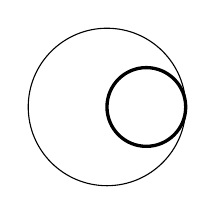
\begin{tikzpicture}[scale=.5]
\draw[very thick] (1,0) circle [radius=1];
\draw[scale=2] (0,0) circle [radius=1]; 
\end{tikzpicture}
\end{tikzshowenvi}
第二行的縮放 \texttt{scale} 是正常圖像的 \(0.5\times 2=1\) 倍。

使用負值來實現“翻轉”效果,以及使用 \tikzkw{scale around} 來指定縮放中心:
\begin{tikzshow}[very thick]
\draw[thin] (0,0) circle [radius=1];
\draw[xscale=-1] (0,0) rectangle (1,1);
\draw[red, xscale=-1] (0,0) rectangle (1,1);
\draw[blue, scale around={1.5:(1,1)}] (0,0) rectangle (1,1);
\end{tikzshow}

注意,縮放命令 \tikzkw{scale} 並不更改對象的屬性,比如點的字體大小、線寬等等。如果想要改變這些,參考\secref{subsec:nodescaling}部分。

\subsubsection{傾斜(slant)*}
傾斜不是一個常用的圖像變換。\tikzz\ 中的傾斜指令是 \tikzkw{xslant} 與 \tikzkw{yslant}。簡單地解釋,\texttt{xslant=k} 會把圖像中座標為 \((x,y)\) 的點變換為 \((x+k\times y, y)\)。
\begin{tikzshow}[very thick,scale=.6]
\draw[help lines] (0,0) grid (4,2);
\draw (0,0) -- (1,1) -- (1,2) -- cycle;
\draw[red, xslant=1.5] (0,0) -- (1,1) -- (1,2) -- cycle;
\draw[blue, xslant=-1] (0,0) -- (1,1) -- (1,2) -- cycle;
\end{tikzshow}

\subsection{裁剪(clip)}
在 \latexline{clip} 命令\RED{之後}的所有繪圖都會只顯示該裁剪視窗中的部分:
\begin{tikzshow}
\clip (0,0) rectangle (1.1, 1.1);
\draw[red, thick] (0,0) circle [radius=1];
\end{tikzshow}

添加 \tikzkw{draw} 選項可以把 \latexline{clip} 命令的“輪廓”繪製出來\footnote{也可使用 \latexline{draw} 命令並將 \tikzkw{clip} 作為參數,還可將兩者作為 \latexline{path} 命令的參數。}:
\begin{tikzshow}
\clip[preaction={draw=red,ultra thick}] (1.2,0) arc [start angle=0, end angle=225, radius=1.2];
\draw (-1,-1) rectangle (1,1);
\draw (-1,1) -- (1,-1);
\end{tikzshow}
上例使用一個非閉合的路徑(圓弧)來裁剪,\tikzz\ 會自動將其首尾連接。其中,\tikzkw{preaction} 選項表示在 \latexline{clip} 命令\RED{之前}先沿該路徑按傳遞給其的參數繪製,之後再創建裁剪視窗;這樣可以實現視窗輪廓的自定義繪製(因為裁剪隻影響其後的繪製命令)。

\subsection{分組(scope)}
\label{subsec:scope}
分組操作允許你對當前組使用參數——這些參數會疊加到全局參數上,並且不影響到組外的對象:
\begin{tikzshowenvi}
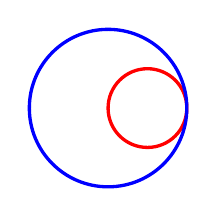
\begin{tikzpicture}[red, very thick, scale=.5]
\draw (1,0) circle [radius=1];
\begin{scope}[blue, scale=2]
\draw (0,0) circle [radius=1];
\end{scope}
\end{tikzpicture}
\end{tikzshowenvi}

\subsection{畫布大小}
命令 \latexline{useasboundingbox} 可以

\section{點(node)與文本}

\subsection{點的座標指定}
使用 \latexline{coordinate} 命令給點命名,便於之後引用。
\begin{tikzshow}
\coordinate (A) at (1,0);
\coordinate (B) at (1,1);
\draw (0,0) -- (A) circle[radius=.5] -- (B) -- cycle;
\end{tikzshow}
\tikzkw{coordinate} 也可以在繪製命令中作為選項使用。

\subsection{點的基本命令}
如需顯式地繪製點(即佔有面積的點),使用 \latexline{node} 命令,或者 \latexline{path} 命令的 \tikzkw{node} 選項,並配合 \tikzkw{draw} 選項。選項 \tikzkw{shape} 用於指定點的繪製方式。
\begin{tikzshow}
\node at (0,0) [shape=circle, draw] (C) {$p_C$};
\node at (1,0) [rectangle, draw, fill=red] {};
\path[yshift=1cm] (0,.5) node[draw] (A) {$p_A$}
     (1,.5) node[draw] (B) {$p_B$};
\draw (A) -- (B) -- (C);
\end{tikzshow}
選項 \tikzkw{shape} 還可賦值為 \texttt{coordinate},這樣在點之間連線時會從點中心開始繪製;但我建議此時直接使用 \tikzkw{coordinate} 命令。

\subsubsection{點的錨點(anchor)}
使用 \tikzkw{anchor} 選項定義錨點位置,可傳入的值是 4 個基本方位(east, west, south, north)、4 個複合方位(south west 等),以及 center。或者你可以依次用 left, right, above, below 來替代四個基本方位:
\begin{tikzshow}
\draw[help lines] (0,0) grid (2,2);
\draw (0,0) node [anchor=south west] {$\beta$};
\node at (0,1) [above right] {Here};
\node at (1,0) [above=2pt] {Hi};
\draw (1,2) node [below right=1pt and 8pt] {$1,0$};
\end{tikzshow}
其中,如果像最後一行給出雙距離參數,需加載 \pkg{positioning} 庫。

也可以直接用數字指定 \tikzkw{anchor} 的角度,\tikzz\ 會自動定位到點邊界上對應角度的位置:
\begin{tikzshow}
\draw (0,0) circle [radius=1];
\foreach \x in {1,...,12} {
  \node at (90-30*\x:1) [anchor=270-30*\x] {\x};
}
\end{tikzshow}

點的命名類似 \latexline{coordinate} 的用法:
\begin{tikzshow}
\path node (a) at (0,0) {}
      node (b) at (1,0) {};
\draw (a) -- (b);
\end{tikzshow}

\subsubsection{點的尺寸}
點的大小用 \tikzkw{inner sep} 指定文字到點邊框的距離,用 \tikzkw{minimum size} 指定邊框的最小尺寸。也可以配合 \tikzkw{text width} 選項指定文本的每行寬度。
\begin{tikzshow}
\tikzset{every node/.style={draw, circle}}
\node (a) {a};
\node[yshift=1cm] (b) {b};
\node[shift={(1,2)}, inner sep=2pt] (c) {c};
\node[xshift=1cm, minimum size=8pt] (d) {d};
\node[shift={(1,1)}, minimum size=8pt, inner sep=0pt] (e) {e};
\end{tikzshow}
注意點 \(d\) 和點 \(e\) 的區別。

\subsection{點的相對放置}
點的相對放置有兩種方式。其一如下例,雙距離語句需要 \pkg{positioning} 庫。
\begin{tikzshow}
\tikzset{every node/.style={draw, circle}}
\draw[help lines] (0,0) grid (3,3);
\node (a) {a};
\node (b) [above=of a] {b};
\node (c) [above right=.5cm and 2cm of b] {c};
\node (d) [below=.5cm of c, on grid] {d};
\draw[red] (b) rectangle (d);
\end{tikzshow}
\tikzkw{on grid} 選項表示從邊框而不是點中心開始計算距離,因此 \(b\) 與 \(d\) 的縱座標不同。另一種方式是使用方位詞結合點的名稱,組成 \texttt{點名\mbox{.}方位詞} 的語法:
\begin{tikzshow}
\node (a) {a};
\node[above] (aa) at (a.north) {a.north};
\end{tikzshow}
上例中的 \tikzkw{above} 選項不是必須的,但往往添加以避免點間的覆蓋。

\subsection{點的旁置文本(label/pin)}
旁置文本(或標籤)可用上一節的語法畫另一個點來實現,但 \tikzkw{label} 或 \tikzkw{pin} 選項更簡潔,會直接在主點旁畫一個旁置點。對同一個主點畫多個 \tikzkw{label} 或 \tikzkw{pin} 都是允許的;它們的區別在於後者會在主點和旁置點之間連一條線。

標籤位置的語法是 \texttt{角度\mbox{:}文本}——它還有一個特殊的角度參數 \texttt{center},會將標籤放在主點的中心處。你也可以通過 \tikzkw{label distance} 或 \tikzkw{pin distance} 選項來指定距離。
\begin{tikzshow}[every node/.style={draw, circle}]
\draw node[pin={[pin distance=.2cm, pin edge={<-, thick}]above right:$a_{p}$}] (a) at (0,0) {a} 
node[label={[red]30:$b'$}] (b) at (0,1) {b} 
node[label=120:$c'$, label=below:$c''$] (c) at (1.5,1) {c};
\end{tikzshow}
上例中甚至給 \tikzkw{label} 傳入了顏色參數。還可以使用 \texttt{every pin, every pin edge} 或 \texttt{every label} 樣式設定默認值。

當點被旋轉時,參數 \tikzkw{absolute} 可以幫助你定位。如果它的值是 \texttt{true} 或缺省,那麼方向不會跟隨點而旋轉,而是始終以紙面做參照:
\begin{tikzshow}
\tikzset{
    every node/.style={draw, rectangle},
    every label/.style={draw=red, font=\footnotesize}
}
\node[rotate=-80,label=right:label] (a) at (0,0) {normal};
\draw[blue, thick] (0,0) -- (-80:1);
\node[rotate=-80,label={[absolute]right:label}] (b) at (1,0) {absolute};
\draw[blue, thick] (1,0) -- +(0:1);
\end{tikzshow}
左側標籤的錨點(位於紅色矩形的左側邊上)在點“normal”右側邊框的中點,而右側標籤的錨點則位於穿過點“absolute”中心的水平向右的線上。\RED{上例中出現了方括號嵌套時,不要忘記添加花括號}。

\subsection{點的沿路徑文本}
\subsubsection{顯示指定}
將 \tikzkw{node} 選項放於對應的點座標之後,稱為顯示(explicitly)指定。

對於沿路徑的文本標記,\tikzz\ 預定義了 7 種位置,分別是 \tikzkw{at start/end}, \tikzkw{(very) near start/end},以及缺省時的 \tikzkw{midway}。
\begin{tikzshow}
\draw (0,0) .. controls (.5,2) .. (1.5,2)
  node[at start] {at start}
  node[midway, sloped, above] {midway}
  node[pos=1, right, text width=3ex] {at end};
\end{tikzshow}
上例中的一些參數:
\begin{para}
\item[sloped] 設置文字基線與圖中此處的切線平行。
\item[pos] 定量化的位置參數\footnote{並不是嚴格的空間分點;而是基於首、尾、控制點間向量計算出速度,取其時間分點。很難精確指定。}。比如預定義的 \tikzkw{very near start} 即為 \(0.125\),\tikzkw{near start} 即為 \(0.25\)。
\end{para}

對於交點指定(\tikzkw{|-} 或 \tikzkw{-|}),中點(\tikzkw{midway})即為垂足:
\begin{tikzshow}
\draw (0,0) |- (2,1) \foreach \p in {0,0.5,1} {
  node[pos=\p] {\p}
};
\end{tikzshow}

不同位置放置文本的場合,使用 \tikzkw{auto} 選項,並可以設定 \texttt{left} 或者 \texttt{right} 參數;選項 \tikzkw{swap} 則允許你將其文本放在對稱位置。注意:這兩個選項\RED{只對沿路徑的放置有效}。
\begin{tikzshow}[scale=.5, every node/.style={circle, inner sep=2pt}]
\foreach \x in {1,...,4} {
  \draw (90-90*\x:2) -- (-90*\x:2)
  node[midway, fill=red!30, auto=left] {\x}
  node[midway, fill=blue!30, auto, swap] {\x};
}
\end{tikzshow}

\subsubsection{隱式指定}
路徑裏點的位置可以隱式(implicitly)指定,放在 \texttt{--} 命令與要連接的點之間即可。只有隱式指定的點才會繼承全局參數(因此隱式指定往往可以省略一些參數,比如 \tikzkw{midway})。例子\cite{tikzmanual}:
\begin{tikzshowenvi}
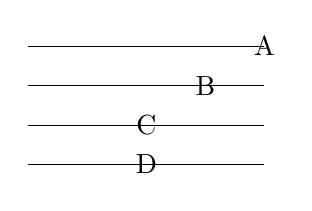
\begin{tikzpicture}[near end]
\draw (0,2.5) -- (3,2.5) node{A};
\draw (0,2) -- node{B} (3,2);
\draw (0,1.5) -- node[midway] {C} (3,1.5);
\draw (0,1) -- (3,1) node[midway] {D} ;
\end{tikzpicture}
\end{tikzshowenvi}
將上述代碼中的 \tikzkw{--} 換成 \tikzkw{to} 也可以;通常後者是個更強的命令,在下一節中也會介紹。

\subsection{點之間的連線}
\label{subsec:connectingnodes}
\subsubsection{基礎連線}
點之間連線會自動檢測點的繪製邊界,主要要三種操作方式:
\begin{enumerate}
\item 在點名稱後增加小數點和方位詞來指定,比如點 a 的左側就用 \texttt{(a.west)};
\item 使用 \texttt{to} 代替 \texttt{--},並附加 \tikzkw{out} 與 \tikzkw{in} 選項。(如果不附加則會畫直線)
\item 使用 \texttt{to} 附加 \tikzkw{bend left/right} 選項。下例中最後一行以 a 到 b 直線方向為角度 0,\texttt{bend left=45} 表示逆時針旋轉 $45$ 度作為 \tikzkw{out} 值,旋轉 $180-45=135$ 度作為 \tikzkw{in} 值。
\end{enumerate}
\begin{tikzshow}
\tikzset{every node/.style={draw,circle}}
\node (a) {a};
\node (b) [below=of a] {b};
\node (c) [left=of b] {c};
\draw[blue, ->] (c.north) .. controls +(up:1) and +(left:1) .. (a.west); 
\draw[red, ->] (c) [out=315, in=225] to (b);
\draw[->] (a) to [bend left=45] (b);
\end{tikzshow}

\subsubsection{繪製到命令(to)}
除了上面提到的 \tikzkw{to} 命令的用法,它還有以下靈活的使用方式:

使用 \tikzkw{edge node} 來給點之間的連接線添加文本。但更好用的是 \tikzkw{edge label} 命令,表示以 \tikzkw{auto} 選項來自動放置文本;如果換成 \tikzkw{edge label'},則表示以 \tikzkw{auto, swap} 選項放置。
\begin{tikzshow}
\coordinate (a);
\coordinate (b) at ($ (a)+(2,1) $);
\draw (a) to[edge node={node [sloped,above] {ab}}] (b);
\draw (a) to[color=red, bend right=45, edge label=auto, edge label'=swap] (b);
\end{tikzshow}

最後,該命令允許用户以 \tikzkw{to path} 選項來指定繪製方式,並用 \latexline{tikztostart} 表示當前 \tikzkw{to} 命令的起始點,\latexline{tikztotarget} 表示終止點,\latexline{tikztonodes} 表示繪製路徑時伴隨的點(可省略)。實質上是添加了一個路徑分組(花括號內的選項不會應用到外部):
\begin{latex}
{[every to, <options>] <path>}
\end{latex}

例子:
\begin{tikzshow}
\tikzset{selfloop/.style={to path={.. controls +(75:1) and +(105:1) .. (\tikztotarget) \tikztonodes}}}
\node (a) {$a$};
\node[right=of a] (b) {$b$};
\node[below=of b] (c) {$c$};
\draw[->] (a) edge (b) (b) edge[selfloop] node[above] {Hi} (b)  edge (c);
\end{tikzshow}
你可能注意到,上例中雖然定義了 \tikzkw{to path},但使用了 \tikzkw{edge} 而不是 \tikzkw{to};實質上兩者的語法有相近之處,但使用 \tikzkw{to} 會導致只有最後一條子路徑有箭頭。

庫 \pkg{topaths} 定義了一些實用的樣式,比如在上例中就可以直接使用它預定義 \tikzkw{loop above}。

\subsubsection{邊命令(edge)}
邊命令的底層形式是,其中 \verb|<path>| 與 \tikzkw{to} 格式相同:
\begin{latex}
\path[every edge, <options>] (\tikztostart) <path>
\end{latex}

因此它將繪製包含同一個點(即 \texttt{\char`\\tikztostart})的所有邊。當你想要給每個點的邊進行定製時,這會十分有用:
\begin{tikzshow}
\tikzset{every node/.style={draw,circle}}
\node (a) {a};
\node (b) [below=of a] {b};
\node (c) [left=of b] {c};
\draw[thick] (c) edge[red, -latex] (b)
    edge[bend left=45] (a)
    edge[blue, <-] (a);
\end{tikzshow}
提醒一下那些熟悉圖論的讀者:別忘了儘管最後一行中邊的箭頭方向是從 a 到 c 的,但仍可以像上面一樣用 c 點的 \tikzkw{edge} 命令來繪製。

你還可以連寫邊命令,並沿邊加上文字:
\begin{tikzshow}
\node foreach \name/\angle in {a/0,b/90,c/180,d/270}
    (\name) at (\angle:1.5) {$\name$};
\path[->] (b) edge node[above right] {$5$} (a)
  edge (c)
(c) edge [-,dashed, blue] node[auto] {auto}
  node[auto, swap] {swap} (a)
  edge (d)
(d) edge [red] node[above,sloped] {very}
  node[below,sloped] {red} (a);
\end{tikzshow}
這裏用到了之前提及的 \tikzkw{auto} 命令。注意,只要 \tikzkw{path} 命令指定了箭頭選項,\tikzkw{edge} 命令繪製的每條邊都有箭頭。

\subsection{點與畫布的縮放}
\label{subsec:nodescaling}


\subsection{作為圖像的點(pic)*}
一段繪圖代碼可能需要複用;如果它比較複雜,可以使用 \latexline{pic} 來重複調用。
\begin{tikzshow}[scale=0.8]
\tikzset{dcircle/.pic={\draw (0,0) circle [x radius=.5, y radius=.8] circle [radius=1];}}
% 兩種調用方式
\draw[help lines] (0,-1) grid (2,2);
\pic at (0,0) {dcircle}; 
\path (2,0) pic {dcircle};
\end{tikzshow}
語法非常類似 \tikzkw{node}。其中 \tikzkw{at} 也可以寫成 \texttt{[at=\{(0,0)\}]} 這種形式。

\tikzkw{pic actions} 選項用於傳入 \texttt{draw, fill, shade, 或 clip} 參數:
\begin{tikzshow}[scale=0.6, transform shape]
\tikzset{circlerect/.pic = {
    \path[pic actions] (.5,.5) circle [radius=.3];
    \draw (0,0) rectangle (1,1);
}}
\draw[red] (0,0) grid (4,2);
\pic [blue, thick] at (.5,.5) {circlerect};
\pic [draw=blue, fill=white] at (2.5,.5) {circlerect};
\end{tikzshow} 
當不傳入 \tikzkw{draw} 選項時,圓的 \latexline{path} 命令是不會繪製的;同時注意,因為繪製矩形的是 \latexline{draw} 命令,因此不受\tikzkw{fill} 選項影響。

插入的 \tikzkw{pic} 中的點可以在外部調用,一個例子:
\begin{tikzshow}
\tikzset{mypic/.pic={
  \draw[blue] (0,0) coordinate (-A)
  -- (1,1) coordinate (-B);
}}

\draw[help lines] (0,0) grid (1,2);
\pic (P) {mypic};
\pic (Q) at (0,1) {mypic};
\draw[red] (P-A) -- (Q-B);
\end{tikzshow}
\tikzkw{pic} 定義時用短橫命名是為了可讀性。調用時語法類似 \tikzkw{node}。

\pkg{quotes} 庫支持以加引號字串的方式傳入參數,作為 \tikzkw{pic text} 選項的值。比如 \texttt{angles} 這個預定義的 \tikzkw{pic}(由 \pkg{angle} 庫支持):
\begin{tikzshow}
\draw (0,-1) coordinate (P1)
  -- (0,0) coordinate (O)
  -- (1,1) coordinate(P2)
  pic [draw, "$\alpha$"] {angle=P1--O--P2};
\end{tikzshow}

一些其他注意:
\begin{feai}
\item 如果有 \texttt{foreach} 語句,\textbf{請放在 \texttt{pic} 定義的首行} 。
\item \tikzkw{pic} 雖説從用法上近似 \tikzkw{node},實質上它是以類似 \tikzz\ \envi{scope} 環境的方式工作的。因此,如果想要其外部的圖像變換對其生效,須添加 \tikzkw{transform shape} 選項於 \envi{tikzpicture} 環境。
\item \tikzkw{pic} 對象也能像 \tikzkw{node} 一樣,沿路徑放置,設置 \tikzkw{at start} 等選項。
\item 將 \tikzkw{pic} 作為選項使用時,添加 \tikzkw{behind path} 或者 \tikzkw{in front of path} 來指定將 \tikzkw{pic} 插入到所在路徑的下方或是上方圖層。
\item 如果你只是臨時使用而不想額外定義,這裏有一個使用 \tikzkw{code} 選項的例子\cite{tikzmanual}:
\begin{tikzshow}
\draw (0,0) .. controls(1,0) and (2,1) .. (3,1)
foreach \t in {0, 0.1, ..., 1} {
  pic [pos=\t] {
    code={\draw circle [radius=2pt];}
  }
};
\end{tikzshow}
注意,本例只有一句語句。句中 \tikzkw{pic} 是 \latexline{draw} 命令的選項。
\end{feai}

\section{路徑(path)}
雖然我們不常直接使用 \latexline{path} 命令,而是使用它的變體 \latexline{draw} 等,但是我們仍然需要介紹一些它的特性。

最常用的情景就是隻聲明點,但卻不顯示地繪製它們:
\begin{tikzshow}
\path coordinate (a)
     coordinate[right=of a] (b)
     coordinate[above=of b] (c);
\draw (a) -- (b) -- (c) -- cycle;
\end{tikzshow}

特別指明,點命令(\tikzkw{node} 或者 \tikzkw{coordinate})總是在路徑繪製結束後再繪製的;它們不是路徑的一部分。

以下路徑命令已在上文(或將在其他小節)進行介紹:
\begin{description}
\item[移動(move-to)指令] 隱式。如 \verb|draw (a) -- (b) (c) -- (d)|,在 b 與 c 間即為移動指令。
\item[直線(line-to)指令] 包括直線指令 \tikzkw{--} 與水平豎直線指令 \tikzkw{|-} 和 \tikzkw{-|}。
\item[曲線(curve-to)指令] 即繪製 \bz\ 曲線的 \tikzkw{.. controls ..} 指令。
\item[繪製到(to)指令] 上文介紹過 \tikzkw{to} 配合 \tikzkw{out, in, bent left} 等命令的用法,參考前文\secref{subsec:connectingnodes}。它實際將指令解釋為以上三種指令之一。
\item[幾何形狀指令] 包括圓或橢圓 \tikzkw{circle}、矩形 \tikzkw{rectangle} 與弧 \tikzkw{arc} 指令。
\item[函數指令*] 包括拋物線 \tikzkw{parabola}、正弦 \tikzkw{sin} 與餘弦 \tikzkw{cos} 指令。更復雜的函數會在
\item[網格指令] 即 \tikzkw{grid} 指令。
\item[圓角指令*] 即 \tikzkw{rounded corners} 與 \tikzkw{sharp corners} 指令。
\item[循環指令] 即 \tikzkw{foreach} 指令,具體可參考\secref{subsec:foreach}部分。
\item[暫存指令] 即 \tikzkw{let} 指令,將數據暫存以供語句之後調用。參考\secref{subsec:nodesdistance}部分。
\item[圖指令*] 即 \tikzkw{graph} 指令,繪製圖、樹、網絡的命令。參考\secref{sec:network}部分。
\item[圖像指令*] 即 \tikzkw{pic} 命令,
\end{description}

本節會介紹除上述指令外的其他路徑指令。

\subsection{路徑分組}
類似與 \envi{scope} 環境,\tikzz\ 允許在路徑中創建一個“分組”,分組中的選項不會影響到分組外部的內容。只需要將想要建立分組的部分用花括號包圍即可:
\begin{tikzshow}
\path coordinate (a)
     coordinate[right=of a] (b)
     coordinate[above=of b] (c)
     coordinate[left=of c] (d);
\draw (a) -- (b) {[rounded corners] -- (c) -- (d) {[sharp corners] -- cycle}};
\end{tikzshow}
注意,並不是所有參數都支持分組。例如,每條路徑只能有一個顏色,因此在分組中指定另一種顏色是無效的。

\subsection{SVG 指令*}
加載 \pkg{svg.path} 庫後,路徑中的 \tikzkw{SVG} 選項允許你使用類似網頁 \texttt{HTML} 中 \texttt{SVG} 的語法進行繪製。這裏不再詳細對 SVG 語法做説明,僅給出一個例子:
\begin{tikzshow}
\draw[fill=red!50] svg {M 0 0 L 10 10 h 20 v -10} -- cycle;
\end{tikzshow}
該庫只支持真正的 \texttt{SVG} 指令集的主要部分,並不是完全涵蓋。

\subsection{繪圖指令(plot)}
該指令用於繪製點較多的圖,也可以從外部文件讀取。

\subsection{計算指令(pgfextra)}
該指令只能用於路徑命令內部,運行到此處時路徑繪製會掛起,直到運行完該命令內部的部分再繼續繪製。一個例子:
\begin{tikzshow}
\newdimen\myloc
\myloc=0cm
\draw (0,\myloc) \pgfextra{\myloc=.5cm}
    circle [radius=\myloc] -- (0,1);
\end{tikzshow}

\section{數學繪製:幾何與函數圖像}
嚴格的幾何學繪圖需要一些特別的命令,比如計算兩點間的距離。而且,通常會使用 \tikzkw{coordinate} 而不是 \tikzkw{node} 命令;因為前者並不佔用面積,這樣畫線時才能保證抵達點所在的中心座標。

\subsection{座標計算}
庫 \pkg{calc} 允許用户使用 \texttt{\$ ... \$} 的形式來計算,並放在一對圓括號中作為座標:
\begin{tikzshow}
\coordinate[label=below:A] (A);
\coordinate[above right=.5 and 1.5 of A, label=right:B] (B);
\draw (A) -- (B);
\draw ($ (A) + (.3,.4) $) circle (.5);
\end{tikzshow}

\subsection{兩點距離計算}
\label{subsec:nodesdistance}
上一節中的半徑值是人工計算的。下例讓 \tikzz\ 計算距離,並用 \tikzkw{let} 選項將其儲存起來,在 \tikzkw{in} 選項的後方進行調用:
\begin{tikzshow}[scale=0.6, transform shape]
\coordinate[label=left:A] (A);
\coordinate[above right=.5 and 1.5 of A, label=right:B] (B);
\draw (A) -- (B);
\draw let \p1 = ($ (B) - (A) $),
         \n{rad} = {veclen(\x1,\y1)}
      in (B) circle[radius=\n{rad}]
         (A) circle[radius=\n{rad}];
\end{tikzshow}
命令 \verb|\p<數字>| 用於存儲向量計算結果,比如 \verb|\p1|。對應的,使用 \verb|\x1| 或者 \verb|\y1| 可以調用向量的兩個座標值。而 \verb|\n<數字>| 則用於存儲數值。此外,命令 \tikzkw{veclen} 用於計算向量的歐式長度 \(\sqrt{x^2+y^2}\)。  

如果不想使用數字命名,可以像上例的存儲數值一樣使用字符串;不過這樣命名需要加上花括號。事實上,已知圓心 $A$ 和圓周上一點 $B$,有更簡單的畫圓方法,參考\secref{subsec:circlethrough}部分的內容。

\subsection{$\lambda$分點與垂線}
\subsubsection{比例分點}
分點是幾何中常用的概念,\pkg{calc} 庫支持像 \pkg{xcolor} 混合顏色類似的命令:\verb|<點A>!<分點比例>![角度]<點B>|,不同的是“角度”會將分點位置繞 A 旋轉一個角度。將它還可以用最後一行中鏈式的方法進行連寫:
\begin{tikzshow}
\coordinate[label=left:A] (A);
\coordinate[above right=.5 and 1.5 of A, label=right:B] (B);
\coordinate (X) at ($ (A)!0.5!(B) $);
\coordinate[label=above:C] (C) at ($ (X)!{sqrt(3)}!90:(B) $);
\path[draw=black, fill=blue!20] (A) -- (B) -- (C) -- cycle;
\node[draw=black, fill=red!20, circle through=(X)] at ($ (A)!0.5!(B)!{tan(30)}!90:(B) $) {};
\end{tikzshow}

\subsubsection{距離分點}
你也可以用(直線段)分點距離代替分點比例,加上單位即可:
\begin{tikzshow}
\coordinate[label=left:A] (A);
\coordinate[above right=.5 and 1.5 of A, label=right:B] (B);
\coordinate (C) at ($ (A)!0.5!(B) $);
\draw ($ (C)!1cm!90:(B) $) edge (B) edge (A)
     edge[dashed] node[above, sloped, font=\footnotesize] {1cm} (C);
\end{tikzshow}

\subsubsection{投影分點(垂線)}
用投影點代替分點比例,則得到該點向連線段的投影:
\begin{tikzshow}
\coordinate[label=left:A] (A);
\coordinate[above right=.5 and 2 of A, label=right:B] (B);
\coordinate[above right=1 and .5 of A, label=above:C] (C);
\draw (A) -- (B) -- (C) -- cycle;
\draw[red] (C) -- ($ (A)!(C)!(B) $);
\end{tikzshow}

\subsection{過某點的圓*}
\label{subsec:circlethrough}
使用 \pkg{through} 庫可以方便地畫出給定圓心和過某點的圓,而不需要做兩點距離計算:
\begin{tikzshow}[scale=0.6]
\coordinate[label=below left:A] (A);
\coordinate[above=1 of A, label=above right:B] (B);
\draw (A) -- (B);
\node[draw, circle through=(B), label=left:C] at (A) {};
\node[draw, circle through=(A), label=right:D] at (B) {};
\end{tikzshow}
注意,\tikzkw{circle through} 僅僅適用於 \tikzkw{node} 命令。

\subsection{交點}
在\secref{subsec:intersection}中已經介紹過交點的使用,包括 \tikzkw{-|} 指令與 \pkg{intersections} 庫的一些用法。這裏的例子更復雜一些,也複習了之前等分點的用法:
\begin{tikzshow}
\tikzset{small/.style={draw, circle, fill=black, inner sep=1pt}}
\coordinate[label=left:A] (A);
\coordinate[above right=.5 and 1.5 of A, label=right:B] (B);
\coordinate[label=below:C] (C) at ($ (A)!0.5!(B) $);
\coordinate (D) at ($ (C)!2!90:(B) $);
\coordinate (E) at ($ (C)!2!-90:(B) $);
\draw (A) -- (B);
\draw[red, name path=Lv] (E) -- (D);
\node[draw, circle through=(B), name path=Ca] at (A) {};
\path[name intersections={of=Lv and Ca, by={[label=above right:D]D, [label=right:E]E}}];
\foreach \x in {A,C,D,E}
  \node[small] at (\x) {};
\end{tikzshow}
注意上例中的 \latexline{path} 命令雖聲明瞭交點,但沒有畫任何內容。

\section{圖與網絡繪製*}
\label{sec:network}

\section{屬性}
\label{sec:tikz-property}

\subsection{線寬}
\tikzz\ 預定義了 7 種線寬,從細到粗是:\tikzkw{ultra thin}, \tikzkw{very thin}, \tikzkw{thin}, \tikzkw{semithick}, \tikzkw{thick}, \tikzkw{very thick}, \tikzkw{ultra thick}。或者利用 \tikzkw{line width} 選項指定。
\begin{tikzshow}
\draw[ultra thin] (0,0) -- (1,0);
\draw[ultra thick] (1,0) -- (2,0);
\draw[line width=10pt] (0,1) -- (2,1);
\end{tikzshow}
初始線寬是 0.4pt;兩個 \tikzkw{ultra} 線寬分別是 0.1pt 與 1.6pt。

\subsection{線型}
\tikzz\ 預定義了 4 種基本線型:\tikzkw{dashed}, \tikzkw{dotted}, \tikzkw{dash dot}, \tikzkw{dash dot dot}。它們還可以配合 \tikzkw{loosely} 或者 \tikzkw{densely} 進行微調。
\begin{tikzshow}
\draw[dashed] (0,0) -- (1,0);
\draw[dotted] (0,-0.5) -- (1,-0.5);
\draw[dash dot] (0,-1) -- (1,-1);
\draw[dash dot dot] (0,-1.5) -- (1,-1.5);
\draw[loosely dashed] (0,-2) -- (1,-2);
\draw[densely dotted] (0,-2.5) -- (1,-2.5);
\end{tikzshow}

如果的確需要深度自定義,請使用 \tikzkw{dash pattern} 自定義線型,並可配合 \tikzkw{dash phase} 指定線型的起始位置。
\begin{tikzshow}
\draw[dash pattern=on .1cm off .25cm on .25cm off .15cm, dash phase=1cm] (0,0) -- (3,0);
\end{tikzshow}

有時你可能會看到一些複雜的裝飾線(需要 \pkg{decorations} 庫),比如:\tikz{\draw [->,decorate,decoration=snake] (0,0) -- (2,0)}。請參考\secref{subsec:deco}。

\subsection{線尾(line cap)*}
如果線寬度較大,不同的線尾 \tikzkw{line cap} 明顯對應不同的效果:
\begin{tikzshow}[every label/.style={font=\footnotesize}]
\foreach \offset/\s in {0/rect, .5cm/butt, 1cm/round} {
    \draw[yshift=\offset,line width=5pt, line cap=\s] (0,0) -- (1,0)  node[label=right:\s] {};
    \draw[yshift=\offset, white] (0,0) -- (1,0);
}
\end{tikzshow}

\subsection{線交(line joint)*}
連續畫線時(非連續畫線處此選項無效),可以設置 \tikzkw{line joint}:
\begin{tikzshow}[every label/.style={font=\footnotesize}]
\foreach \offset/\s in {0/round, 1.25cm/bevel, 2.5cm/miter} {
    \draw[xshift=\offset,line width=5pt, line join=\s] (0,0) -- (.5,1) node[label=above:\s] {} -- (1,0)  ;
}
\end{tikzshow}
其中 \tikzkw{miter} 線交在鋭角時會產生一個非常“尖”的效果,可以設置 \tikzkw{miter limit} 參數來設置一個角度值,使小於該角度的 \tikzkw{miter} 線交自動轉變為 \tikzkw{bevel} 形式。

\subsection{箭頭}
\tikzz\ 中的箭頭使用的細節多到可以單獨開一個章節,但我並不想全部詳盡地介紹。用大於或小於號表示箭頭的指向,用豎線表示是否加上截斷符號。一些基本的樣例:
\begin{tikzshow}
\draw[->|] (1,3) -- (2,3);
\draw[stealth-] (1,2) -- (2,2);
\draw[->,>=stealth, line width=3pt] (1,1) arc [start angle=90, end angle=30, radius=1];
\draw[<->] (.5,4) -- (.5,0) -- (2.5,0);
\end{tikzshow}
其中,用 \texttt{>=stealth} 或 \texttt{-stealth} 的方式指定了箭頭末端的類型為 \texttt{stealth}。你也可以將它們作為整個 \envi{tikzpicture} 環境的參數進行傳遞。

\tikzz\ 的 \pkg{arrows.meta} 庫包含很多箭頭,讀者可以自行查閲。

\subsection{繪製顏色}
在繪製網格一節,已經使用過 \texttt{lightgray} 作為網格的繪製顏色;當時省略了 \tikzkw{color} 選項。該選項設定\RED{除了 shading 外的所有}顏色,包括繪製、填充等:
\begin{tikzshow}
\path[draw,fill,red!50] (0,0) -- (1,0) circle[radius=.5];
\end{tikzshow}
注意:單獨使用 \latexline{draw} 或者 \latexline{fill} 只會執行繪製或填充其一,除非詳細指定局部的參數。

可以使用 \tikzkw{draw} 來單獨指定繪製的顏色:
\begin{tikzshow}
\draw[draw=red!50!white, ultra thick] (0,0) rectangle (1,1);
\end{tikzshow}
其中,雙感嘆號加數字是表示插值比例為 0.5;\pkg{xcolor} 宏包支持該語法。常用的顏色包括:
\begin{tikzshow}
\tikzset{every pin/.style={pin distance=.5cm, font=\footnotesize, inner sep=0pt}}
\draw (0,0) circle[radius=1];
\foreach \c[count=\i] in {red,green,blue,cyan,magenta,yellow,black,
lightgray,gray,darkgray,white,brown,
lime,olive,orange,pink,purple,teal,violet}
\node[circle,draw=black, fill=\c, pin={[pin edge={draw=\c, thick}] 90-360/19*\i:\c}] at (90-360/19*\i:1cm) {};
\end{tikzshow}

在 \tikzz\ 環境內部,還可以使用 \latexline{colorlet} 或者 \latexline{definecolor} 自定義顏色(它們實際上是 \TeX\ 指令),例如:
\begin{latex}
\colorlet{linecolor}{red!60!black}
\definecolor{fillcolor}{rgb}{1,0.5,1}
\end{latex}

\subsection{單色填充}
填充命令 \latexline{fill} 只能使用於閉合區域,\textbf{且不繪製區域邊界}。你可以在一般繪製命令的末尾添加 \tikzkw{cycle} 來創建一個閉合對象:
\begin{tikzshow}
\fill[green] (0,0) -- (1,0) -- (1,1) -- cycle;
\end{tikzshow}

在填充的同時繪製\footnote{準確地説,\latexline{filldraw} 命令是先繪製再填充。},使用 \latexline{filldraw} 命令,並分別指定繪製和填充顏色:
\begin{tikzshow}
\filldraw[draw=black, fill=cyan] (0,0) -- (2,0) arc (0:30:2);
\end{tikzshow}
\tikzkw{filldraw} 填充的區域會比用 \tikzkw{fill} 稍大一些,因為前者考慮了線寬。

要了解填充的細節,需要介紹兩個區域特性:
\subsubsection{非零區域}
該特性是默認的區域特性。\tikzz\ 使用計數器的方式來區分路徑的內部與外部。對於某點的判斷,它會從該點發射一條到無窮遠的射線;如果沿途的路徑是從左到右(順時針)地與這條射線相交,那麼計數器加一;反之減一。最後計數器如果是零,那麼該點在路徑外部;否則,它在區域內部。

下例逆時針地繪製了小矩形、順時針地繪製了完全圍住小矩形的大矩形。這樣小矩形的內部被識別為“外部”,因此未被填充。
\begin{tikzshow}
\filldraw[fill=blue!50] (0,0) -- (0,.5) -- (1,.5) -- (1,0) -- cycle
  (-.5,-.5) -- (1.5,-.5) -- (1.5,1) -- (-.5,1) -- cycle;
\end{tikzshow}

\subsubsection{奇偶區域}
奇偶區域也會發射一條射線,但只要遇到路徑就會計數器加一。利用區域的奇偶性填充,使用 \tikzkw{even odd rule}:
\begin{tikzshow}
\fill[even odd rule, blue] (0,0) -- (2,0.5) -- (1,1) circle (0.25);
\end{tikzshow}

\subsection{圖案與圖像填充*}
在指定了 \tikzkw{pattern} 選項時,它會自動進行填充操作(即使你使用的是 \latexline{draw} 命令)。要使用圖案填充,請加載 \pkg{patterns} 庫。
\begin{tikzshow}
\draw[pattern=dots, pattern color=red] (0,0) rectangle (1,1);
\end{tikzshow}

圖像填充允許你使用外部圖像,或者一般的 \tikzz\ 命令。注意配合 \tikzkw{path picture bounding box} 使用。
\begin{tikzshow}

\end{tikzshow}

\subsection{漸變填充*}
使用 \latexline{shade} 命令控制漸變填充,

\subsection{透明度*}
p169

\subsection{雙線*}
雙線選項在某些場合也是實用的。可以用 \tikzkw{double distance} 指定雙線內間距(默認 0.6pt),或者用 \tikzkw{double distance between line centers} 指定雙線的中心間距。
\begin{tikzshow}
\draw[double] (0,0) -- (1,1);
\draw[draw=white, double=cyan] (1,0) -- (0,1);
\draw[double distance=1pt] (1.2,0) -- (1.2,.5);
\draw[double distance=1pt,thick] (1.2,.5) -- (1.2,1);
\end{tikzshow}
上例的 \tikzkw{draw} 指定為白色,實質創造一種“從上方穿過”的效果。

還有一個特殊的雙線選項 \tikzkw{double equal sign distance},可以將雙線間距設置成與當前字體的等號($=$)間距一致。

\section{樣式與高級控制}
\subsection{樣式(style)}
如果某種屬性需要用來反覆作圖,可以把它自定義為樣式:

上文中出現過的 \texttt{help lines},就是 \tikzz\ 預定義的一種樣式。其相當於於:
\begin{latex}
\begin{tikzpicture}[help lines/.style={line width=0.2pt,gray}]
...
\end{tikzpicture}
\end{latex}

你也可以在進入 \tikzz\ 環境後(或在文檔導言區),使用 \latexline{tikzset} 命令來定義。

\subsection{循環語句(foreach)}
\label{subsec:foreach}
\tikzz\ 支持循環語句,這一點對於科技繪圖來説十分重要。
\begin{tikzshow}[place/.style={circle, draw, fill=black, minimum size=5pt, inner sep=0pt}]
\foreach \x in {1,2,3} {
    \node at (\x, 0) [place] {};
    \draw (\x, 0) circle [radius=1/\x];
}
\end{tikzshow}

有時候我們需要循環一個等差數列,這時候使用 \ldots\ 即可。\tikzz\ 會將 \(a,b,\ldots,c\) 識別為從 \(a\) 到 \(c\) 以 \(b-a\) 為公差的等差數列;如果你不指定 \(b\),那麼默認以 \(1\) 為公差。
\begin{tikzshow}[place/.style={circle, draw, fill=black, minimum size=5pt, inner sep=0pt}]
\foreach \x in {1,1.5,...,3,4} {
    \node at (\x, 0) [place] {};
    \draw (\x, 0) circle [radius=\x/8];
}
\end{tikzshow}
上例中的 \(4\) 不在數列內,這樣寫是允許的。數列後也可以接另一個數列。

大部分需要知道“循環到列表第幾個”的場合,都可以配合移動畫筆或相對座標命令實現:
\begin{tikzshow}[scale=.5]
\draw[red] (0,0) grid (3,3);
\foreach \x/\y in {0,1/2,2}
  \draw (\x, \y) +(.5,.5) circle [radius=.4];
\end{tikzshow}
上例同時循環了多個變量,中間用斜線分隔;它們分別按照列表中斜線分隔後的對應值進行循環。如果某一位置的列表提供值的個數小於變量的個數,那麼“多出”的變量將都取最後一個值。

此外,如果 \latexline{foreach} 內部只有一條語句,像上例一樣不加花括號也可以。

\subsection{圖層*}
一般情況不會用到此指令。但有時你需要先畫完上層的內容才能確定下層元素的尺寸,這時候可能需要圖層\cite{tikzmanual}(需要 \pkg{backgrounds} 庫):
\begin{tikzshow}
\tikzset{every node/.style={draw,circle,inner sep=.1cm, minimum size=.8cm}}
\foreach \x/\pos in {{a/(0,0)},{b/(1.5,0)},{c/(1,-1)}}
    \node (\x) at \pos {\x};
\draw (b.east) .. controls +(0:1) and +(0:1) .. (c.east);
\begin{scope}[on background layer]
    \node[draw=none,fill=lightgray, rectangle, fit=(b) (c)] {};
\end{scope}
\end{tikzshow}
上例中還使用了 \pkg{fit} 庫,用來創建一個“遮蓋”點 b 和點 c 的背景點——這個點的矩形邊框被 \tikzkw{fit} 命令處理成圖中的大小。

\subsection{裝飾*(decorations)}
\label{subsec:deco}
最簡單的裝飾是蛇形線\cite{tikzmanual},需要 \pkg{decorations.pathmorphing} 庫:
\begin{tikzshow}
\draw[->,decorate,decoration=snake] (0,0) -- (2,0);
\end{tikzshow}

通常,我們希望在線段結束就終止裝飾(否則會蛇形繪製到線段末尾,這可能引起困惑)。下面是一個複雜的例子:
\begin{tikzshow}
\draw[->, decorate, decoration={snake,amplitude=.4mm,segment length=4mm,post length=2mm}] (0,0) -- (3,0)
    node[above, align=center, midway, text width=2.5cm, font=\footnotesize] {
        multiline text controlled by \texttt{text width} option of \textcolor{blue}{node}
    };
\end{tikzshow}
大部分的參數都比較好理解。\tikzkw{amplitude} 控制波動的強弱,\tikzkw{segment length} 控制一個週期的長度,\tikzkw{post length} 控制在終點之前何處結束裝飾。

\subsection{隨機數*}
\tikzz\ 使用 \tikzkw{rand} 來生成從 $-1$ 到 $1$ 的隨機數(服從均勻分佈);如果使用 \pkg{calc},你還可以在指定座標時使用 \texttt{(\$...\$)} 並在其中做座標計算: 
\begin{tikzshow}
\makeatletter\def\pgfcurrentseed{
  \pgfmathparse{\pgfmath@rnd@z}\pgfmathresult
}\makeatother
\coordinate [label=left:$A$] (A) at (.5*rand,.5*rand);
\draw (0,0) node[below=1] {\pgfcurrentseed} circle [radius=1];
\coordinate [label=left:$B$] (B) at ($ (0,0) + (rand,rand)$);
\path (0,0) node[above=1] {\pgfcurrentseed};
\end{tikzshow}
上例中在 \TeX\ 底層中使用 pgf 命令從 \latexline{pgfmath@rnd@z} 中讀取當前隨機數種子的值,並賦給自定義命令。每次使用 \tikzkw{rand} 命令都會改變隨機數種子的值。

\subsection{外部數據文件*}

\section{實用範例}
\label{sec:tikz-eg}
本節通過例子的方式,向讀者展示 \tikzz\ 的常用情形。